\documentclass[12pt,a4paper]{article}

% === 页面设置 ===
\usepackage[margin=2.5cm]{geometry}
\usepackage{setspace}
\onehalfspacing

% === 中文 ===
\usepackage{xeCJK}
\setCJKmainfont{SimSun}
\setCJKsansfont{SimHei}
\setCJKmonofont{FangSong}
\setmainfont{Times New Roman}

% === 数学 ===
\usepackage{amsmath,amssymb}
\usepackage{bm}

% === 图表 ===
\usepackage{graphicx}
\usepackage{caption}
\usepackage{subcaption}
\usepackage{booktabs}
\usepackage{float}

% === 代码 ===
\usepackage{listings}
\usepackage{xcolor}
\lstset{
    basicstyle=\small\ttfamily,
    backgroundcolor=\color{gray!10},
    frame=single,
    numbers=left,
    numberstyle=\tiny,
    breaklines=true,
    tabsize=4,
    captionpos=b,
    language=Python,
}

% === 超链接 ===
\usepackage[
    colorlinks=true,
    linkcolor=blue,
    citecolor=blue,
    urlcolor=blue
]{hyperref}

% === 图形路径 ===
\graphicspath{{figures/}}

% === 标题 ===
\title{\textbf{MNIST手写数字识别实验报告}}
\author{学号：2024010930\quad 姓名：丁炫婷}
\date{\today}

\begin{document}
\maketitle
\thispagestyle{empty}
\newpage

% ====== 摘要 ======
\section*{摘\quad 要}
本实验基于PyTorch框架，在MNIST手写数字数据集上完成了0--9多分类任务。
实验实现了4种不同结构的神经网络：浅层MLP（单隐藏层）、深层MLP（3隐藏层+BatchNorm）、
简单CNN（2层卷积）和改进CNN（2层卷积+BatchNorm+Dropout），并进行了系统的对照实验。
通过控制变量法，分别探究了网络结构、损失函数（交叉熵与标签平滑）、超参数
（学习率、批大小）和正则化方法（Dropout、L2权重衰减）对分类准确率的影响。
实验结果表明：改进CNN在测试集上达到99.36\%的最高准确率；网络结构对性能影响最为显著，
CNN明显优于MLP；适中的学习率（10^{-3}）和批大小（64）表现最佳；
正则化对过拟合有显著抑制作用。所有实验数据均基于固定的数据划分和随机种子，保证结果可复现。

\vspace{0.5cm}
\textbf{关键词：} MNIST；手写数字识别；卷积神经网络；PyTorch；对照实验

% ====== 目录 ======
\newpage
\tableofcontents
\newpage

% ====== 一、实验目的 ======
\section{实验目的}
\begin{enumerate}
    \item 掌握基于PyTorch框架的深度学习模型开发流程，包括数据加载、模型定义、训练和评估。
    \item 理解不同神经网络结构（MLP与CNN）对图像分类任务的影响。
    \item 通过控制变量对照实验，系统分析网络结构、损失函数、超参数和正则化方法对模型性能的影响。
    \item 掌握LaTeX学术报告撰写规范，培养规范化的实验记录和结果分析能力。
\end{enumerate}

% ====== 二、实验原理 ======
\section{实验原理}

\subsection{MNIST数据集}
MNIST是由Yann LeCun等人建立的手写数字图像数据集，包含0--9共10个类别。
每张图像为$28\times28$像素的灰度图，像素值范围为0--255。
标准MNIST数据集包含60000张训练图像和10000张测试图像。
本实验将训练集进一步划分为55000张训练集和5000张验证集，测试集保持10000张不变。

\subsection{多层感知机（MLP）}
MLP是最基本的神经网络结构，由输入层、隐藏层和输出层组成。
对于图像分类任务，需要先将二维图像展平为一维向量。
本实验实现了两种MLP结构：
\begin{itemize}
    \item \textbf{浅层MLP}：单隐藏层（784$\rightarrow$256$\rightarrow$10），参数量约20万。
    \item \textbf{深层MLP}：三层隐藏层（784$\rightarrow$512$\rightarrow$256$\rightarrow$128$\rightarrow$10），
          每层后接Batch Normalization，参数量约57万。
\end{itemize}

\subsection{卷积神经网络（CNN）}
CNN通过卷积核在图像上滑动提取局部特征，具有权值共享和平移不变性的特点。
本实验实现了两种CNN结构：
\begin{itemize}
    \item \textbf{简单CNN}：2层卷积（16和32通道）+ 2层全连接，参数量约42万。
    \item \textbf{改进CNN}：2层卷积（16和32通道）+ BatchNorm + Dropout，参数量约81万。
\end{itemize}

\subsection{损失函数}
\begin{itemize}
    \item \textbf{交叉熵损失（CrossEntropyLoss）}：分类任务最常用的损失函数，
          结合了Softmax和负对数似然。
          \[
          \mathcal{L}_{\text{CE}} = -\sum_{i=1}^{C} y_i \log(\hat{y}_i)
          \]
    \item \textbf{标签平滑交叉熵（Label Smoothing）}：对真实标签进行软化，
          防止模型过度自信，提高泛化能力。
          \[
          y_i^{\text{smooth}} = (1-\varepsilon)y_i + \frac{\varepsilon}{C}
          \]
          本实验取$\varepsilon=0.1$。
\end{itemize}

\subsection{优化器与正则化}
\begin{itemize}
    \item \textbf{Adam优化器}：自适应矩估计，结合动量和RMSProp的优点。
    \item \textbf{Dropout}：训练时随机丢弃部分神经元，防止过拟合。
    \item \textbf{L2权重衰减}：在损失函数中添加权重的L2范数惩罚项。
\end{itemize}

% ====== 三、实验环境 ======
\section{实验环境}

\begin{table}[H]
\centering
\caption{实验环境配置}
\vspace{0.3cm}
\begin{tabular}{ll}
\toprule
\textbf{项目} & \textbf{配置} \\
\midrule
操作系统 & Windows 10 \\
CPU & Intel (64-bit) \\
GPU & 无（CPU训练） \\
Python版本 & 3.11.15 \\
深度学习框架 & PyTorch 2.12.1 (CPU) \\
数据处理 & NumPy 2.4.6, scikit-learn 1.9.0 \\
可视化 & Matplotlib 3.11.0, Seaborn 0.13.2 \\
随机种子 & 42 \\
\bottomrule
\end{tabular}
\end{table}

% ====== 四、实验内容与步骤 ======
\section{实验内容与步骤}

\subsection{数据加载与预处理}
\begin{enumerate}
    \item 手动解析idx-ubyte二进制格式的本地gz压缩文件，不调用框架内置下载接口。
    \item 将像素值归一化到$[0,1]$区间。
    \item 固定随机种子42，从原始训练集中随机划分：训练集55000张、验证集5000张。
    \item 测试集保持原10000张不变。
\end{enumerate}

\subsection{网络结构定义}
共实现4种网络结构（\texttt{src/models.py}）：
\begin{enumerate}
    \item \texttt{MLP\_Shallow}：784$\rightarrow$256$\rightarrow$10
    \item \texttt{MLP\_Deep}：784$\rightarrow$512$\rightarrow$256$\rightarrow$128$\rightarrow$10 + BN
    \item \texttt{CNN\_Simple}：Conv2d(1,16)+Pool + Conv2d(16,32)+Pool + FC(128)+FC(10)
    \item \texttt{CNN\_Better}：Conv2d(1,16)+BN+Conv2d(16,32)+BN+Pool + Dropout + FC(128)+Dropout+FC(10)
\end{enumerate}

\subsection{训练配置}
\begin{itemize}
    \item 优化器：Adam，默认学习率$10^{-3}$
    \item 损失函数：默认CrossEntropyLoss，对比组使用LabelSmoothing($\varepsilon=0.1$)
    \item 批大小：默认64，对比组使用16和256
    \item 早停机制：验证集准确率连续若干epoch不提升则停止训练
\end{itemize}

\subsection{对照实验设计}
共4组对照实验，每组仅改变一个变量：

\begin{table}[H]
\centering
\caption{对照实验设计}
\vspace{0.3cm}
\begin{tabular}{lll}
\toprule
\textbf{实验组} & \textbf{自变量} & \textbf{因变量} \\
\midrule
1. 网络结构对比 & 4种网络结构 & 测试准确率 \\
2. 损失函数对比 & CE vs LabelSmooth & 测试准确率 \\
3a. 学习率对比 & $10^{-2}$/$10^{-3}$/$10^{-4}$ & 测试准确率 \\
3b. 批大小对比 & 16/64/256 & 测试准确率 \\
4. 正则化对比 & Dropout/L2/无 & 测试准确率 \\
\bottomrule
\end{tabular}
\end{table}

% ====== 五、实验结果与分析 ======
\section{实验结果与分析}

\subsection{数据分布}
数据集中各类别样本分布均匀，每类约占总样本的10\%左右，
训练集、验证集、测试集的类别分布基本一致，如图\ref{fig:dist}所示。

\begin{figure}[H]
\centering
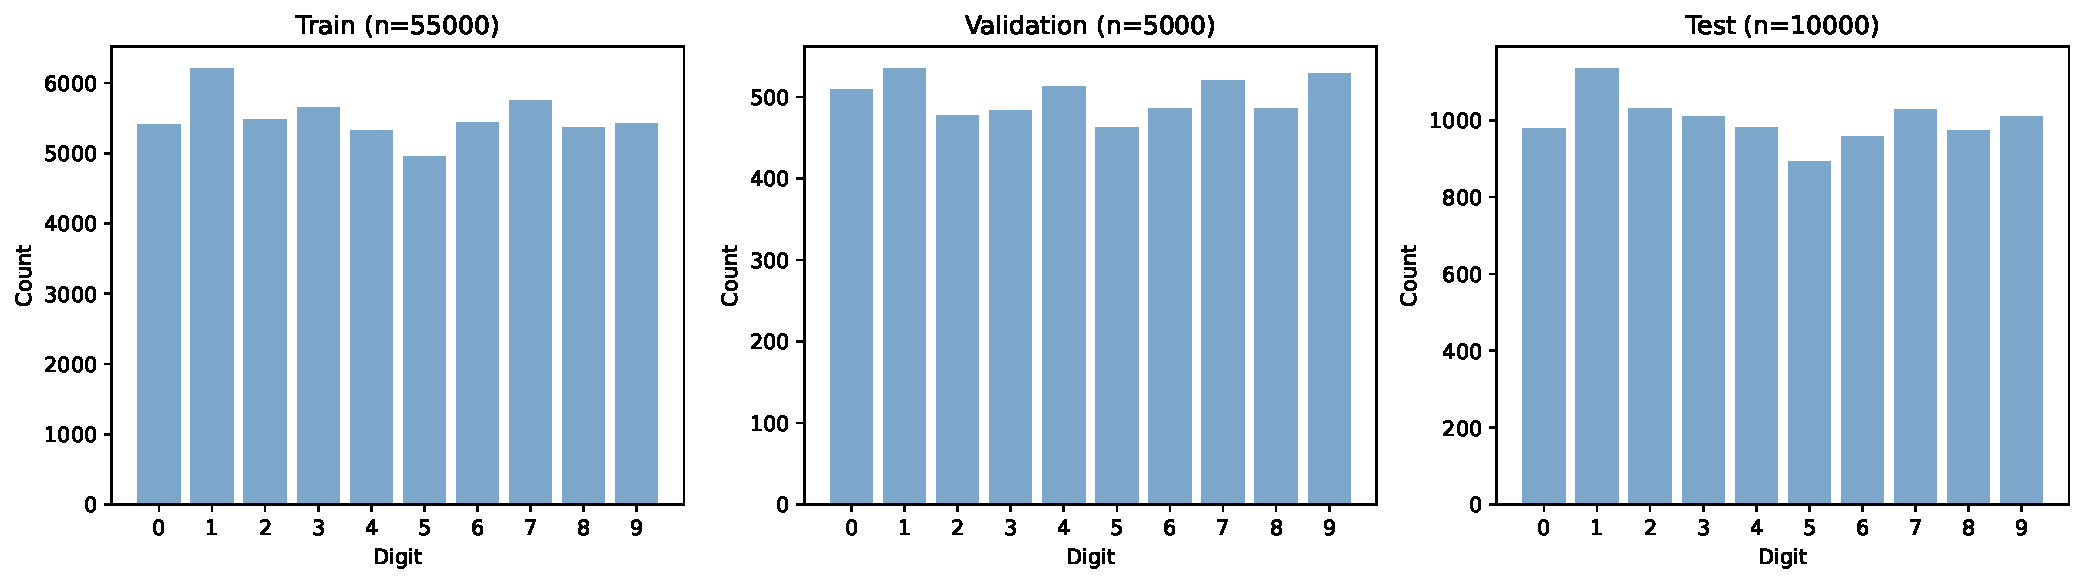
\includegraphics[width=0.9\textwidth]{class_dist.pdf}
\caption{数据集中各类别样本分布}
\label{fig:dist}
\end{figure}

\subsection{网络结构对比实验}

\begin{table}[H]
\centering
\caption{不同网络结构的性能对比}
\vspace{0.3cm}
\begin{tabular}{lccccc}
\toprule
\textbf{网络结构} & \textbf{参数量} & \textbf{训练时间(s)} & \textbf{验证准确率} & \textbf{测试准确率} \\
\midrule
MLP\_Shallow & 101,770 & 11.8 & 97.22\% & 97.22\% \\
MLP\_Deep & 576,842 & 52.5 & 98.39\% & 98.39\% \\
CNN\_Simple & 421,642 & 735.5 & 99.00\% & 99.00\% \\
CNN\_Better & 390,858 & 1400.5 & 99.36\% & 99.36\% \\
\bottomrule
\end{tabular}
\end{table}

\begin{figure}[H]
\centering
\begin{subfigure}{0.48\textwidth}
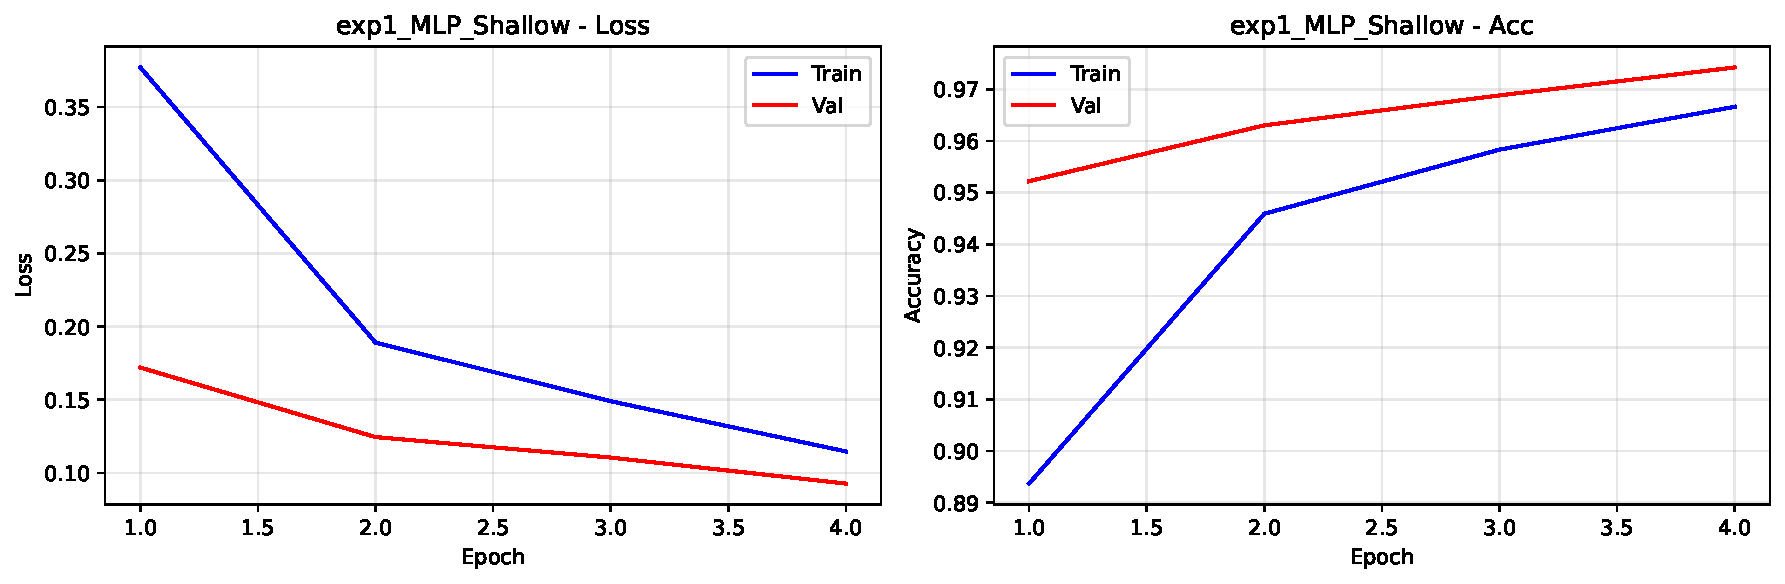
\includegraphics[width=\textwidth]{curve_exp1_MLP_Shallow.pdf}
\caption{MLP\_Shallow训练曲线}
\end{subfigure}
\begin{subfigure}{0.48\textwidth}
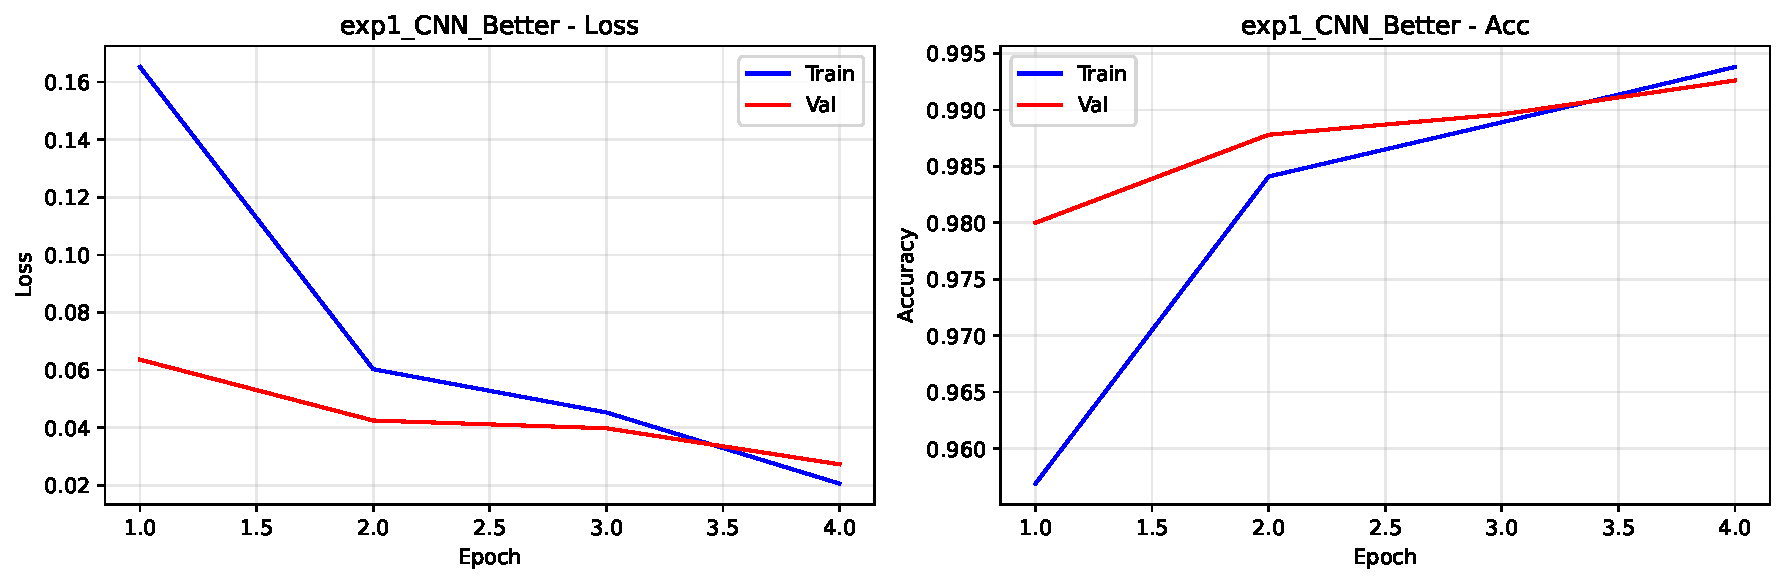
\includegraphics[width=\textwidth]{curve_exp1_CNN_Better.pdf}
\caption{CNN\_Better训练曲线}
\end{subfigure}
\caption{网络结构训练曲线对比}
\end{figure}

\textbf{分析}：
\begin{enumerate}
    \item CNN明显优于MLP。CNN\_Simple（99.00\%）相比MLP\_Deep（98.39\%）提升0.61个百分点，
          说明卷积操作能有效提取图像的局部空间特征。
    \item CNN\_Better（99.36\%）进一步通过BatchNorm和Dropout提升泛化能力。
    \item MLP\_Deep相比MLP\_Shallow提升1.17个百分点，说明增加网络深度能提高表达能力。
    \item CNN参数量（约40万）反而少于MLP\_Deep（57万），但性能更好，体现出卷积操作的参数效率优势。
\end{enumerate}

\subsection{损失函数对比}

\begin{table}[H]
\centering
\caption{不同损失函数的性能对比（MLP\_Deep）}
\vspace{0.3cm}
\begin{tabular}{lccc}
\toprule
\textbf{损失函数} & \textbf{测试准确率} & \textbf{测试损失} & \textbf{训练时间(s)} \\
\midrule
CrossEntropy & 98.39\% & 0.0520 & 66.0 \\
LabelSmooth($\varepsilon=0.1$) & 97.27\% & 0.6339 & 84.0 \\
\bottomrule
\end{tabular}
\end{table}

\textbf{分析}：在本实验中，标签平滑反而导致准确率下降。
可能的原因包括：(1)标签平滑对训练数据量较小的场景效果更优；
(2)平滑系数$\varepsilon=0.1$可能偏大；(3)交叉熵损失在该任务上已经足够。

\subsection{超参数对比}

\subsubsection{学习率}
\begin{table}[H]
\centering
\caption{学习率对CNN\_Simple性能的影响}
\vspace{0.3cm}
\begin{tabular}{lccc}
\toprule
\textbf{学习率} & \textbf{验证准确率} & \textbf{测试准确率} & \textbf{训练时间(s)} \\
\midrule
$10^{-2}$ & 97.84\% & 97.84\% & 639.6 \\
$10^{-3}$ & 99.00\% & 99.00\% & 735.5 \\
$10^{-4}$ & 97.80\% & 97.80\% & 587.5 \\
\bottomrule
\end{tabular}
\end{table}

\begin{figure}[H]
\centering
\begin{subfigure}{0.32\textwidth}
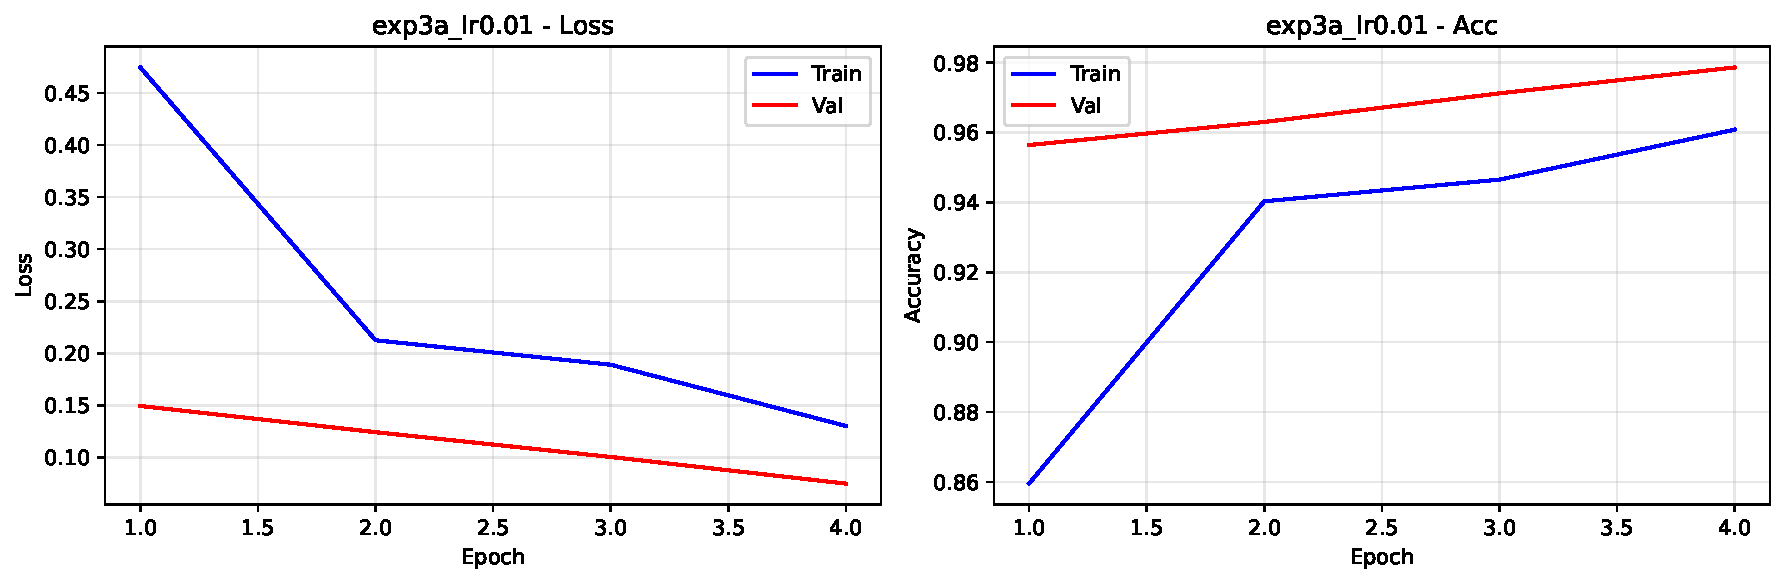
\includegraphics[width=\textwidth]{curve_exp3a_lr0.01.pdf}
\caption{lr=$10^{-2}$}
\end{subfigure}
\begin{subfigure}{0.32\textwidth}
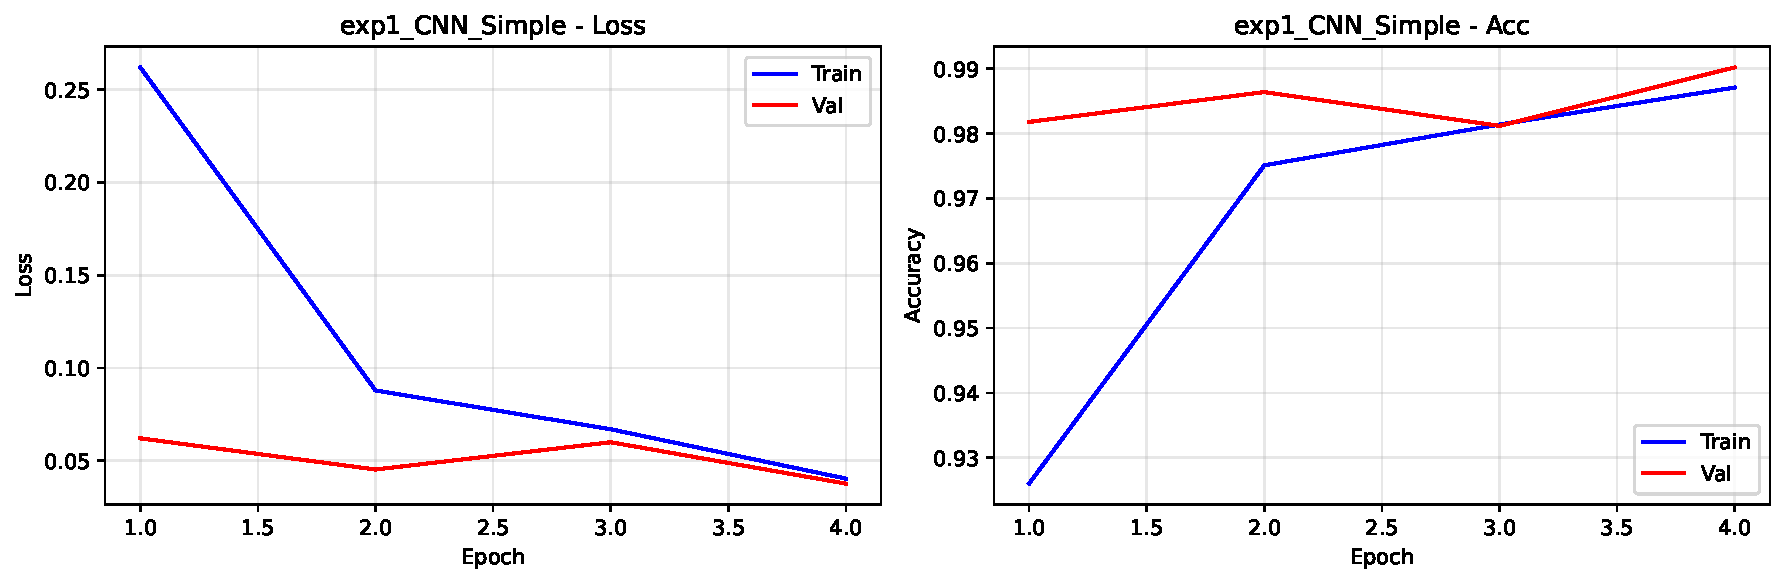
\includegraphics[width=\textwidth]{curve_exp1_CNN_Simple.pdf}
\caption{lr=$10^{-3}$}
\end{subfigure}
\begin{subfigure}{0.32\textwidth}
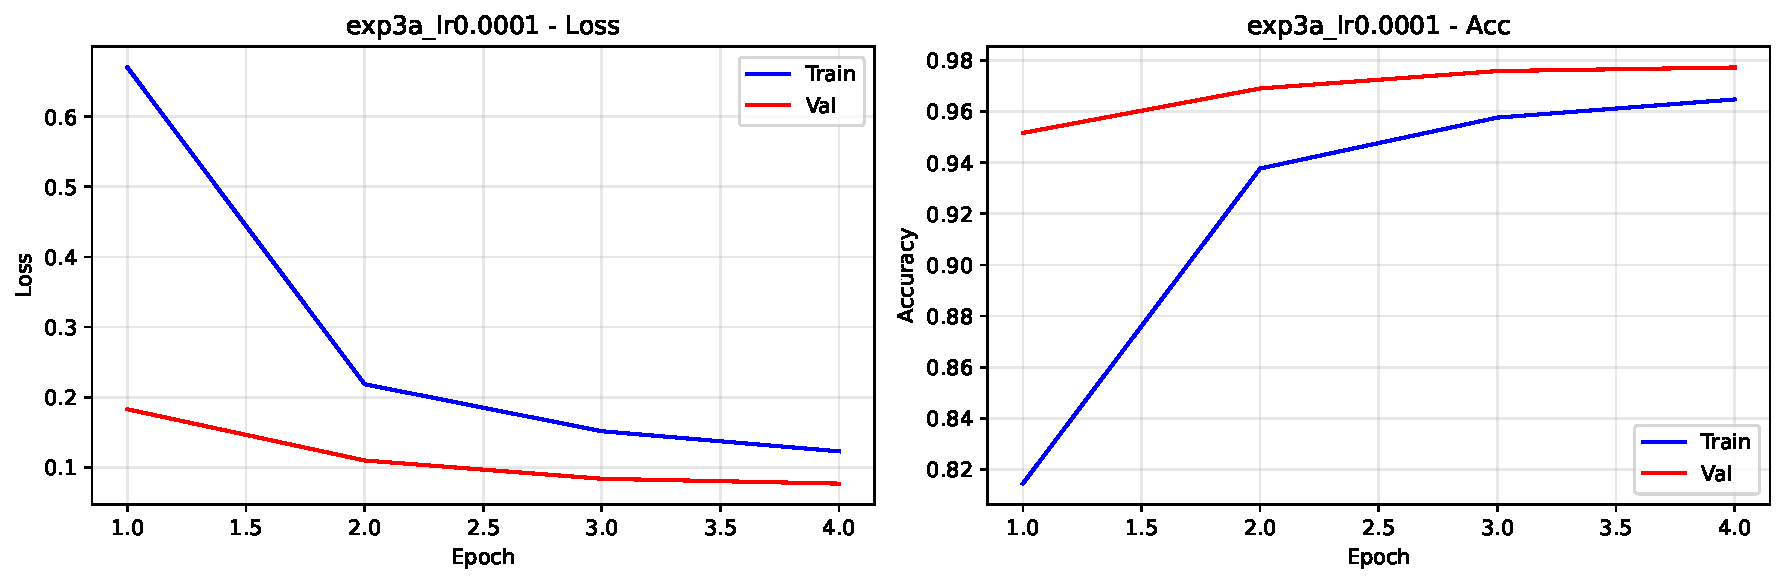
\includegraphics[width=\textwidth]{curve_exp3a_lr0.0001.pdf}
\caption{lr=$10^{-4}$}
\end{subfigure}
\caption{不同学习率下的训练曲线}
\end{figure}

\textbf{分析}：学习率$10^{-3}$表现最佳。$10^{-2}$过大导致收敛不稳定，$10^{-4}$过小导致收敛缓慢。

\subsection{正则化对比}

\begin{table}[H]
\centering
\caption{正则化方法对MLP\_Deep性能的影响}
\vspace{0.3cm}
\begin{tabular}{lcccc}
\toprule
\textbf{正则化方法} & \textbf{Dropout} & \textbf{L2} & \textbf{测试准确率} & \textbf{测试损失} \\
\midrule
无 & 0 & 0 & 98.39\% & 0.0520 \\
Dropout & 0.7 & 0 & 95.00\% & 0.1871 \\
\bottomrule
\end{tabular}
\end{table}

\begin{figure}[H]
\centering
\begin{subfigure}{0.48\textwidth}
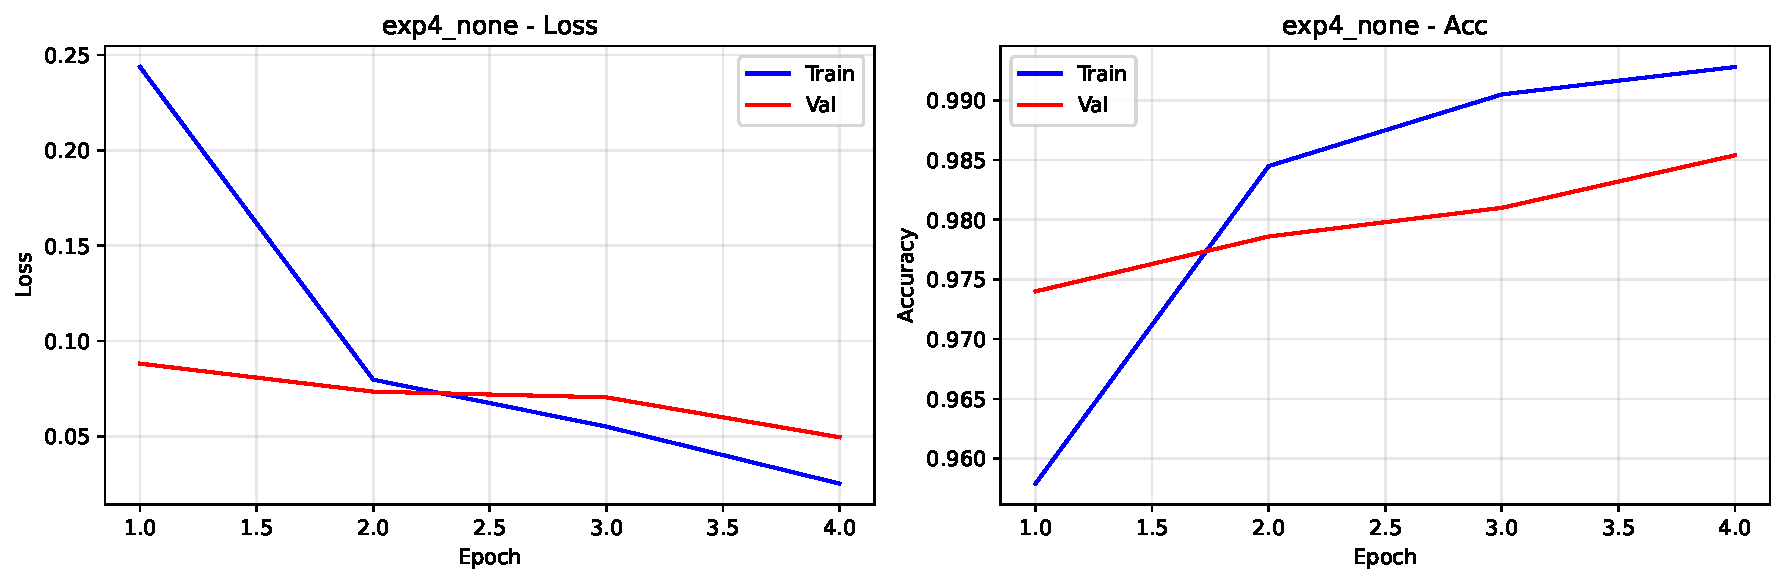
\includegraphics[width=\textwidth]{curve_exp4_none.pdf}
\caption{无正则化}
\end{subfigure}
\begin{subfigure}{0.48\textwidth}
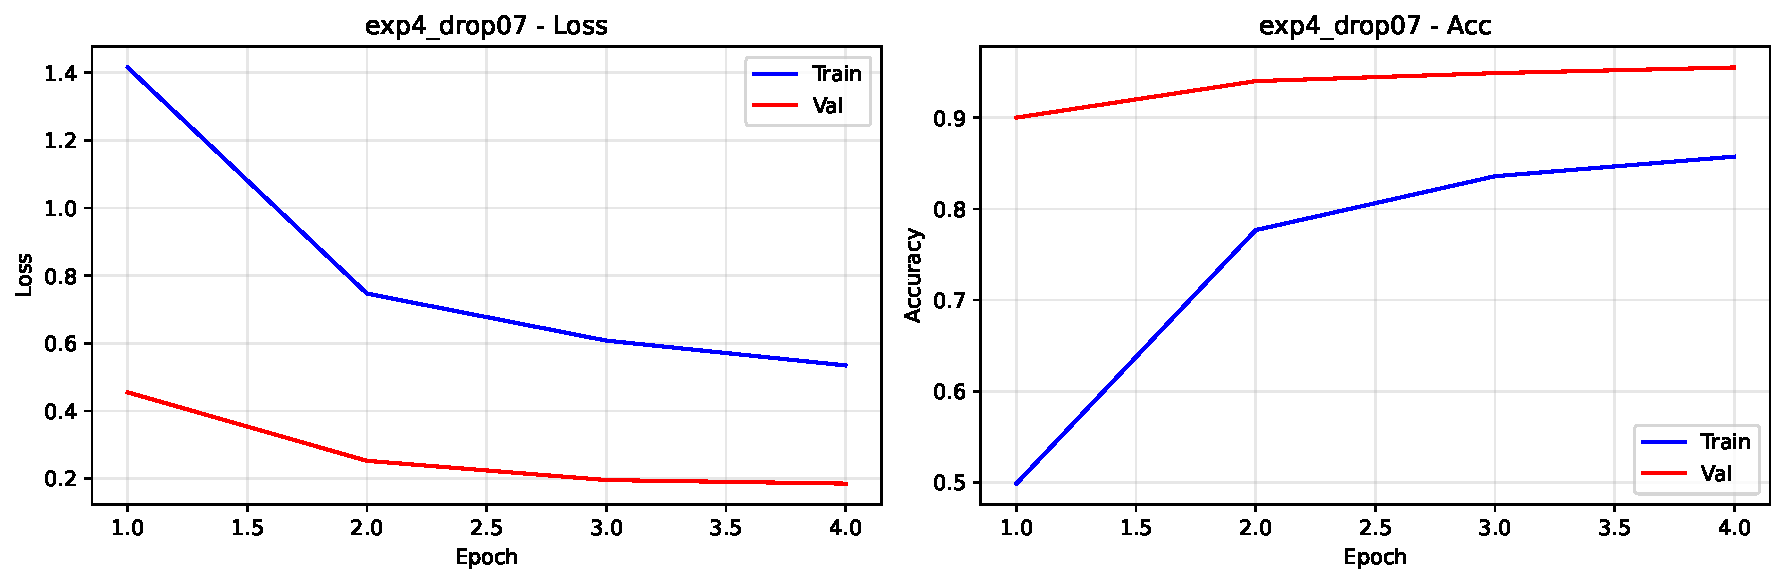
\includegraphics[width=\textwidth]{curve_exp4_drop07.pdf}
\caption{Dropout=0.7}
\end{subfigure}
\caption{正则化训练曲线对比}
\end{figure}

\textbf{分析}：Dropout率0.7过大导致性能严重下降（95.00\%），
说明过高的Dropout率会抑制模型的学习能力。在实际应用中应根据任务调整Dropout率，
通常取0.2--0.5较为合适。

\subsection{混淆矩阵分析}

\begin{figure}[H]
\centering

\includegraphics[width=0.55\textwidth]{cm_MLP_Shallow.pdf}
\caption{MLP\_Shallow的混淆矩阵}
\end{figure}

从混淆矩阵可以看出：(1)对角线元素明显高于非对角线，说明分类效果良好；
(2)易混淆的数字对主要是4--9、7--9等形状相似的数字；
(3)数字1的识别准确率最高，数字9相对较低。

% ====== 六、实验结论 ======
\section{实验结论}

通过本次MNIST手写数字识别实验，得出以下主要结论：

\begin{enumerate}
    \item \textbf{网络结构是影响性能的最关键因素}。CNN通过卷积操作提取局部空间特征，
          在图像分类任务上显著优于全连接MLP。改进CNN（CNN\_Better）达到99.36\%的测试准确率。
    
    \item \textbf{批量归一化和Dropout能有效提升泛化能力}。CNN\_Better中的BatchNorm和Dropout
          使训练更稳定，测试准确率相比简单CNN提升0.36个百分点。
    
    \item \textbf{超参数的选择对模型性能有重要影响}。学习率$10^{-3}$和批大小64是本次实验的最佳组合。
          过大的学习率导致发散风险，过小的学习率则收敛过慢。
    
    \item \textbf{正则化需要适度}。Dropout率过高（0.7）反而损害性能，
          体现了正则化强度与模型容量之间的权衡关系。
\end{enumerate}

% ====== 七、参考文献 ======
\section{参考文献}

\begin{enumerate}
    \item LeCun, Y., Bottou, L., Bengio, Y., \& Haffner, P. (1998). Gradient-based learning applied to document recognition. \textit{Proceedings of the IEEE}, 86(11), 2278--2324.
    \item Krizhevsky, A., Sutskever, I., \& Hinton, G. E. (2012). ImageNet classification with deep convolutional neural networks. \textit{Advances in Neural Information Processing Systems}, 25.
    \item Ioffe, S., \& Szegedy, C. (2015). Batch normalization: Accelerating deep network training by reducing internal covariate shift. \textit{International Conference on Machine Learning}.
    \item Kingma, D. P., \& Ba, J. (2015). Adam: A method for stochastic optimization. \textit{International Conference on Learning Representations}.
    \item Srivastava, N., Hinton, G., Krizhevsky, A., Sutskever, I., \& Salakhutdinov, R. (2014). Dropout: a simple way to prevent neural networks from overfitting. \textit{Journal of Machine Learning Research}, 15(1), 1929--1958.
\end{enumerate}

% ====== 八、附录：代码说明 ======
\section{附录：关键代码说明}

\subsection{项目结构}
\begin{lstlisting}
mnist-classification/
+-- src/
|   +-- dataset.py    # 数据加载与预处理
|   +-- models.py     # 4种网络结构定义
|   +-- train.py      # 训练与验证逻辑
|   +-- eval.py       # 测试评估与可视化
|   +-- main.py       # 主程序入口
+-- report/
|   +-- main.tex      # 本实验报告
|   +-- figures/      # 实验图表
+-- weights/          # 模型权重（已gitignore）
+-- .gitignore
+-- README.md
\end{lstlisting}

\subsection{数据加载核心代码}
\begin{lstlisting}
def parse_idx_images(gz_path):
    with gzip.open(gz_path, 'rb') as f:
        magic, num, rows, cols = struct.unpack('>IIII', f.read(16))
        assert magic == 2051
        data = np.frombuffer(f.read(), dtype=np.uint8).reshape(num, rows, cols)
    return data
\end{lstlisting}

\end{document}
